% Two ways past the wall -- research overview slides (both directions).
% Compile from research/:  pdflatex slides.tex  (twice)
% Non-technical by design: each direction gets "the idea", "why it should
% work", "the evidence", and "status". Numbers come from the committed
% benchmarks (findings.tex, gpu/README.md).
\documentclass[aspectratio=169,11pt]{beamer}
\usepackage[T1]{fontenc}
\usepackage{lmodern}
\usepackage{tikz}
\usetikzlibrary{positioning,decorations.pathreplacing}
\usepackage{booktabs}

% ---------- palette (validated for accessibility, light surface) ----------
\definecolor{ink}{HTML}{22262E}        % near-black, blue-biased
\definecolor{paper}{HTML}{FCFCFB}
\definecolor{mutedink}{HTML}{5C6470}
\definecolor{copper}{HTML}{B76F28}     % direction A: stabilizer rank
\definecolor{teal}{HTML}{2B8FB2}       % direction B: GPU batching
\definecolor{violet}{HTML}{5B50B5}     % "clifft today" in comparisons
\definecolor{faint}{HTML}{E9E8E3}

% ---------- quiet beamer ----------
\setbeamertemplate{navigation symbols}{}
\setbeamercolor{background canvas}{bg=paper}
\setbeamercolor{normal text}{fg=ink}
\setbeamercolor{structure}{fg=ink}
\setbeamercolor{frametitle}{fg=ink,bg=paper}
\setbeamerfont{frametitle}{series=\bfseries,size=\Large}
\setbeamertemplate{frametitle}{%
  \vspace{1.1em}{\usebeamerfont{frametitle}\insertframetitle}\\[-0.35em]
  {\color{framerule}\rule{0.14\textwidth}{2.2pt}}\vspace{0.2em}}
\setbeamertemplate{itemize item}{\raisebox{0.12em}{\color{framerule}\rule{0.5em}{0.14em}}}
\setbeamertemplate{itemize subitem}{\raisebox{0.12em}{\color{mutedink}\rule{0.35em}{0.12em}}}
\setbeamertemplate{footline}{%
  \hfill{\color{mutedink}\scriptsize\insertframenumber\,/\,\inserttotalframenumber}\hspace{1em}\vspace{0.6em}}
\setlength{\leftmargini}{1.1em}

% per-section accent for the title underline
\colorlet{framerule}{ink}
\newcommand{\accentA}{\colorlet{framerule}{copper}}
\newcommand{\accentB}{\colorlet{framerule}{teal}}
\newcommand{\accentO}{\colorlet{framerule}{ink}}

\newcommand{\ket}[1]{\lvert #1 \rangle}
\newcommand{\punch}[1]{{\color{framerule}\bfseries #1}}
\newcommand{\takeaway}[1]{%
  \vfill{\color{framerule}\rule{\textwidth}{0.6pt}}\\[0.35em]
  {\small\itshape #1}}

\title{Two ways past the wall}
\author{}
\date{}

\begin{document}

% ================================================================ title
\begin{frame}
  \vspace{1.6em}
  {\color{mutedink}\scriptsize CLIFFT RESEARCH \,\textperiodcentered\, JULY 2026}\\[0.8em]
  {\Huge\bfseries Two ways past the wall}\\[0.5em]
  {\large Extending clifft beyond its $2^k$ limit}\\[2.2em]
  \begin{columns}[T]
    \begin{column}{0.46\textwidth}
      {\color{copper}\rule{0.5\textwidth}{2.2pt}}\\[0.3em]
      {\bfseries A \,\textperiodcentered\, Stabilizer-rank backend}\\
      {\small\color{mutedink} change the \emph{representation}:\\ pay for magic, not for dimensions}
    \end{column}
    \begin{column}{0.46\textwidth}
      {\color{teal}\rule{0.5\textwidth}{2.2pt}}\\[0.3em]
      {\bfseries B \,\textperiodcentered\, GPU shot batching}\\
      {\small\color{mutedink} change the \emph{hardware use}:\\ run thousands of shots abreast}
    \end{column}
  \end{columns}
\end{frame}

% ================================================================ clifft in 30s
\accentO
\begin{frame}{clifft in thirty seconds}
  \begin{columns}[T]
    \begin{column}{0.52\textwidth}
      \begin{itemize}
        \item Clifford gates are ``easy'': tracked \punch{symbolically}, essentially free, at any width.
        \item Only \emph{magic} ($T$ gates) forces real amplitudes: the dense $2^k$ \punch{active block}.
        \item $k$ = how much magic is live at once --- usually far below the qubit count.
      \end{itemize}
    \end{column}
    \begin{column}{0.44\textwidth}
      \centering
      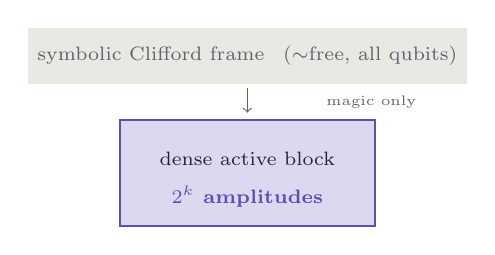
\begin{tikzpicture}[scale=0.9]
        % frame band
        \fill[faint] (-0.5,2.2) rectangle (5.7,3.0);
        \node[color=mutedink,font=\scriptsize] at (2.6,2.6) {symbolic Clifford frame \, ($\sim$free, all qubits)};
        % active block
        \fill[violet!22] (0.8,0.2) rectangle (4.4,1.7);
        \draw[violet,thick] (0.8,0.2) rectangle (4.4,1.7);
        \node[color=ink,font=\scriptsize] at (2.6,1.15) {dense active block};
        \node[color=violet,font=\scriptsize\bfseries] at (2.6,0.62) {$2^k$ amplitudes};
        \draw[->,mutedink] (2.6,2.15) -- (2.6,1.8);
        \node[color=mutedink,font=\tiny] at (4.35,1.95) {magic only};
      \end{tikzpicture}
    \end{column}
  \end{columns}
  \takeaway{One engine, two tiers: symbolic where physics allows it, dense only where it must be.}
\end{frame}

% ================================================================ the wall
\begin{frame}{The wall: $2^k$ doubles with every step}
  \begin{columns}[T]
    \begin{column}{0.5\textwidth}
      \vspace{0.4em}
      \begin{itemize}
        \item Memory doubles per unit of $k$: \punch{$k=30 \Rightarrow 16$ GB}, $k=40 \Rightarrow 16$ TB.
        \item The compiler already fights hard for small $k$ --- what still lands large is \emph{genuinely} dense.
        \item So: \punch{what do we do when $2^k$ itself is the cost?}
      \end{itemize}
    \end{column}
    \begin{column}{0.46\textwidth}
      \centering
      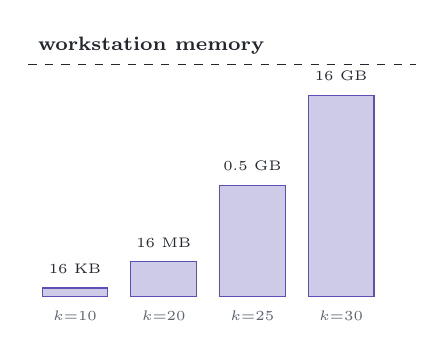
\begin{tikzpicture}[scale=0.88]
        \foreach \i/\h/\lab in {0/0.12/{$k{=}10$},1/0.5/{$k{=}20$},2/1.6/{$k{=}25$},3/2.9/{$k{=}30$}}{
          \fill[violet!30] (\i*1.28,0) rectangle (\i*1.28+0.95,\h);
          \draw[violet] (\i*1.28,0) rectangle (\i*1.28+0.95,\h);
          \node[font=\tiny,color=mutedink] at (\i*1.28+0.475,-0.28) {\lab};}
        \node[font=\tiny,color=ink] at (0.475,0.4) {16 KB};
        \node[font=\tiny,color=ink] at (1.755,0.78) {16 MB};
        \node[font=\tiny,color=ink] at (3.035,1.88) {0.5 GB};
        \node[font=\tiny,color=ink] at (4.315,3.18) {16 GB};
        \draw[ink,dashed] (-0.2,3.35) -- (5.4,3.35);
        \node[font=\scriptsize\bfseries,color=ink,anchor=west] at (-0.2,3.62) {workstation memory};
      \end{tikzpicture}
    \end{column}
  \end{columns}
  \takeaway{Two independent bets on what to do about it --- one mathematical, one architectural.}
\end{frame}

% ================================================================ A: idea
\accentA
\begin{frame}{A \,\textperiodcentered\, The idea: pay for magic, not for dimensions}
  \begin{columns}[T]
    \begin{column}{0.52\textwidth}
      \begin{itemize}
        \item Low-magic states are secretly simple: a \punch{short sum of stabilizer ``recipes''}, a few KB each.
        \item Like storing an image as a few overlapping patterns instead of every pixel.
        \item Cliffords are cheap on recipes; only $T$'s multiply them; \punch{measurements shrink them back}.
      \end{itemize}
    \end{column}
    \begin{column}{0.44\textwidth}
      \centering
      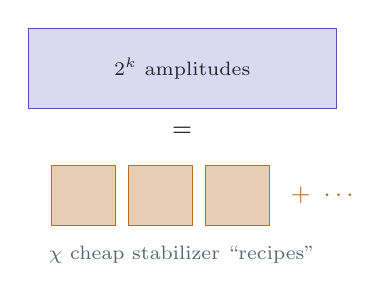
\begin{tikzpicture}[scale=0.85]
        \fill[violet!22] (0,1.9) rectangle (4.6,3.1);
        \draw[violet] (0,1.9) rectangle (4.6,3.1);
        \node[font=\scriptsize,color=ink] at (2.3,2.5) {$2^k$ amplitudes};
        \node[font=\small] at (2.3,1.55) {$=$};
        \foreach \i/\c in {0/1.0,1/0.62,2/0.3}{
          \fill[copper!35] (\i*1.15+0.35,0.15) rectangle (\i*1.15+1.3,1.05);
          \draw[copper] (\i*1.15+0.35,0.15) rectangle (\i*1.15+1.3,1.05);}
        \node[font=\small,color=copper,anchor=west] at (3.78,0.6) {$+\ \cdots$};
        \node[font=\scriptsize,color=mutedink] at (2.3,-0.28) {$\chi$ cheap stabilizer ``recipes''};
      \end{tikzpicture}
    \end{column}
  \end{columns}
  \takeaway{The cost driver becomes the amount of magic $t$, not the dimension $2^k$.}
\end{frame}

% ================================================================ A: why it works
\begin{frame}{A \,\textperiodcentered\, Why it should work}
  \begin{columns}[T]
    \begin{column}{0.52\textwidth}
      \begin{itemize}
        \item An optimal $T$-split keeps the recipe count at \punch{$2^{0.228\,t}$} --- far slower growth than $2^k$.
        \item A \punch{tunable} error $\delta$ lets you keep only a random sample. Measured: error $=0.50\,\delta$, on the nose.
        \item Same language clifft already speaks: frame $+$ measurement collapse.
      \end{itemize}
    \end{column}
    \begin{column}{0.44\textwidth}
      \centering
      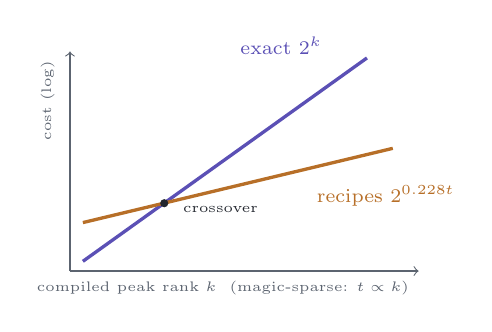
\begin{tikzpicture}[scale=0.82]
        \draw[->,mutedink] (0,0) -- (5.4,0) node[below left,font=\tiny,color=mutedink]{compiled peak rank $k$ \ (magic-sparse: $t \propto k$)};
        \draw[->,mutedink] (0,0) -- (0,3.4) node[rotate=90,anchor=south east,font=\tiny,color=mutedink,yshift=2pt]{cost (log)};
        \draw[violet,very thick] (0.2,0.15) -- (4.6,3.30) node[anchor=south east,font=\scriptsize,color=violet,pos=0.88,yshift=6pt]{exact $2^{k}$};
        \draw[copper,very thick] (0.2,0.75) -- (5.0,1.90) node[anchor=north west,font=\scriptsize,color=copper,pos=0.72,yshift=-2pt]{recipes $2^{0.228 t}$};
        \fill[ink] (1.46,1.05) circle (1.8pt);
        \node[font=\tiny,color=ink,anchor=west] at (1.60,0.95) {crossover};
      \end{tikzpicture}
    \end{column}
  \end{columns}
  \takeaway{Trade exactness you can measure for reach you cannot otherwise have.}
\end{frame}

% ================================================================ A: extent
\begin{frame}{A \,\textperiodcentered\, Under the hood: stabilizer extent}
  \begin{columns}[T]
    \begin{column}{0.52\textwidth}
      \begin{itemize}
        \item Each $T$ gate is a sum of two \emph{Clifford} moves: $T = \alpha\,I + \beta\,S$, with $|\alpha|+|\beta| = 2^{0.114}$ --- provably the cheapest split.
        \item $t$ $T$'s $\Rightarrow$ $2^t$ branches, but their total weight is only $2^{0.114\,t}$. Its square --- the \punch{stabilizer extent $2^{0.228\,t}$} --- is the real price.
        \item Keep a \punch{weight-sampled $k \approx 2^{0.228\,t}/\delta^2$} of the branches: within $\delta$ of the true state, unbiased --- that is the measured $0.50\,\delta$ dial.
      \end{itemize}
    \end{column}
    \begin{column}{0.44\textwidth}
      \centering
      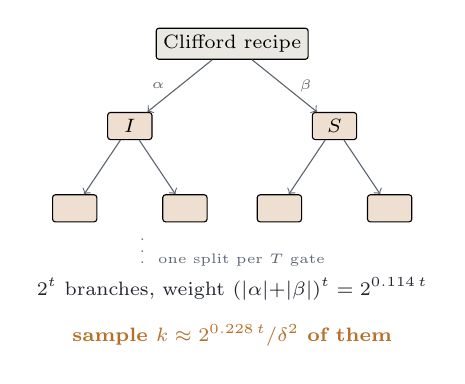
\begin{tikzpicture}[yscale=0.95,
          b/.style={draw, rounded corners=1pt, fill=copper!22, inner sep=2.5pt,
                    minimum width=16pt, font=\scriptsize},
          w/.style={font=\tiny, color=mutedink}]
        \node[b, fill=faint] (r) at (2.6,3.4) {Clifford recipe};
        \node[b] (l) at (1.3,2.3) {$I$};
        \node[b] (s) at (3.9,2.3) {$S$};
        \draw[->,mutedink] (r) -- (l) node[w,midway,left=2pt] {$\alpha$};
        \draw[->,mutedink] (r) -- (s) node[w,midway,right=2pt] {$\beta$};
        \node[b] (n1) at (0.6,1.2) {\phantom{$I$}};
        \node[b] (n2) at (2.0,1.2) {\phantom{$I$}};
        \node[b] (n3) at (3.2,1.2) {\phantom{$I$}};
        \node[b] (n4) at (4.6,1.2) {\phantom{$I$}};
        \draw[->,mutedink] (l) -- (n1);
        \draw[->,mutedink] (l) -- (n2);
        \draw[->,mutedink] (s) -- (n3);
        \draw[->,mutedink] (s) -- (n4);
        \node[w] at (2.6,0.72) {$\vdots$ \ one split per $T$ gate};
        \node[font=\scriptsize, color=ink] at (2.6,0.12)
          {$2^t$ branches, weight $(|\alpha|{+}|\beta|)^t = 2^{0.114\,t}$};
        \node[font=\scriptsize\bfseries, color=copper] at (2.6,-0.5)
          {sample $k \approx 2^{0.228\,t}/\delta^2$ of them};
      \end{tikzpicture}
    \end{column}
  \end{columns}
  \takeaway{$2^t$ branches, but only $2^{0.228\,t}$ of weight --- and weight is all you pay.}
\end{frame}

% ================================================================ A: architecture
\begin{frame}{A \,\textperiodcentered\, How it fits: one compiler, two executors}
  \centering
  \vspace{-0.2em}
  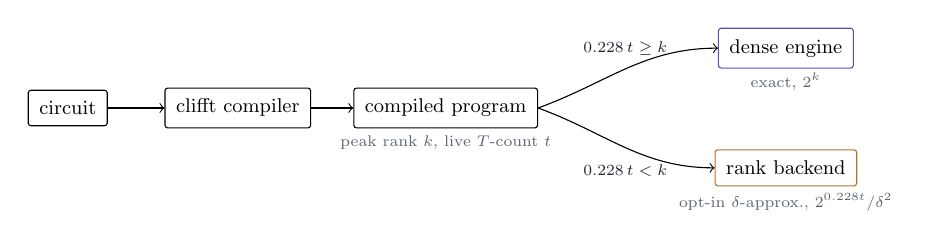
\begin{tikzpicture}[scale=0.8, every node/.append style={transform shape},
    box/.style={draw, rounded corners=1pt, inner sep=5pt, font=\small},
    sub/.style={font=\scriptsize, color=mutedink},
    lbl/.style={font=\scriptsize\itshape, color=ink}]
    \node[box] (circ) at (0,0) {circuit};
    \node[box] (comp) at (2.7,0) {clifft compiler};
    \node[box] (meta) at (6.0,0) {compiled program};
    \node[sub] at (6.0,-0.55) {peak rank $k$, live $T$-count $t$};
    \node[box, draw=violet] (dense) at (11.4,0.95) {dense engine};
    \node[sub] at (11.4,0.42) {exact, $2^{k}$};
    \node[box, draw=copper] (chf) at (11.4,-0.95) {rank backend};
    \node[sub] at (11.4,-1.5) {opt-in $\delta$-approx., $2^{0.228 t}/\delta^2$};
    \draw[->] (circ) -- (comp);
    \draw[->] (comp) -- (meta);
    \draw[->] (meta.east) to[out=20,in=180] (dense.west);
    \draw[->] (meta.east) to[out=-20,in=180] (chf.west);
    \node[lbl] at (8.85,0.95) {$0.228\,t \ge k$};
    \node[lbl] at (8.85,-1.0) {$0.228\,t < k$};
  \end{tikzpicture}
  \vspace{-0.2em}
  \begin{itemize}
    \item Both cost exponents are known \punch{before anything runs} --- dispatch is a one-line comparison, per program.
    \item \punch{Wired, not just proposed}: the rank backend runs clifft's optimized circuits; exact clifft stays the default, the rank backend is an explicit opt-in with an error dial $\delta$.
  \end{itemize}
  \takeaway{clifft compiles; the cheaper engine runs --- on the same optimized circuit.}
\end{frame}

% ================================================================ A: generality
\begin{frame}{A \,\textperiodcentered\, Not an IQP trick: any Clifford$+T$ circuit}
  \begin{itemize}
    \item The fast sampler needs all magic in \punch{one up-front layer} --- IQP (our commuting benchmark family) has that shape by construction; most circuits scatter their $T$'s throughout.
    \item The fix: teleport each in-line $T$ onto a helper qubit --- \emph{any} circuit becomes product-magic, with \punch{no penalty for interleaving}.
    \item \punch{Composes with the compiler}: gadgetize the optimized IR --- pay the \emph{live} $T$-count. Measured: 32 raw $T$'s $\to$ 10, error $5.8\times$ smaller at the same budget.
    \item Tested on circuits whose answer is known \emph{by construction} (hidden shift): up to \punch{96 qubits}, right answer in seconds.
    \item Often clifft still wins such circuits outright --- and the dispatch rule \emph{knows in advance}.
  \end{itemize}
  \takeaway{Generality at the product-magic price --- validated end to end against exact references.}
\end{frame}

% ================================================================ A: episodic
\begin{frame}{A \,\textperiodcentered\, Recycled magic: pay per episode, not per program}
  \begin{itemize}
    \item Long computations \punch{recycle} magic: the block grows, is measured out, grows again --- ``episodes''. Total magic grows with runtime; \punch{per-episode magic stays bounded}.
    \item Run one episode at a time: pay $2^{\,\text{per-episode}}$, not $2^{\,\text{total}}$, with \punch{zero extra error}. Measured: \punch{72 qubits at $\le\!400$ recipes} where whole-circuit needs $2^{72}$.
    \item Compressing further also works (measured, honest limits) --- the dispatcher prices it.
  \end{itemize}
  \takeaway{The circuit's rhythm --- magic in, magic measured out --- is itself a computational resource.}
\end{frame}

% ================================================================ A: circuits
\begin{frame}{A \,\textperiodcentered\, The circuits behind the numbers}
  \begin{columns}[T]
    \begin{column}{0.48\textwidth}
      \centering
      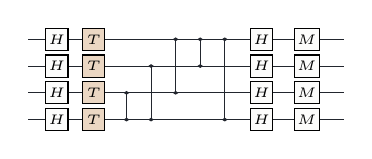
\begin{tikzpicture}[xscale=0.52, yscale=0.34,
          g/.style={draw, fill=paper, inner sep=1pt, minimum size=8pt, font=\tiny},
          t/.style={g, fill=copper!28}]
        \foreach \y in {0,...,3} \draw[ink] (0.3,\y) -- (8.0,\y);
        \foreach \y in {0,...,3} \node[g] at (1.0,\y) {$H$};
        \foreach \y in {0,...,3} \node[t] at (1.9,\y) {$T$};
        \foreach \x/\a/\b in {2.7/0/1, 3.3/0/2, 3.9/1/3, 4.5/2/3, 5.1/0/3}{
          \filldraw[ink] (\x,\a) circle (1.3pt);
          \filldraw[ink] (\x,\b) circle (1.3pt);
          \draw[ink] (\x,\a) -- (\x,\b);}
        \foreach \y in {0,...,3} \node[g] at (6.0,\y) {$H$};
        \foreach \y in {0,...,3} \node[g] at (7.1,\y) {$M$};
      \end{tikzpicture}\\[1pt]
      {\scriptsize\punch{Dense IQP} --- the stress test}\\
      {\tiny\color{mutedink} IQP = ``instantaneous quantum polynomial'': a standard hard commuting family; compiles to peak rank $n/2$}\\[0.9em]
      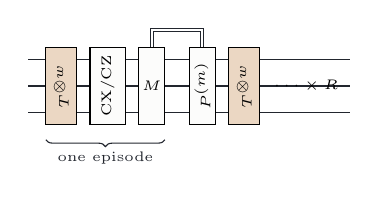
\begin{tikzpicture}[xscale=0.56, yscale=0.34,
          g/.style={draw, fill=paper, inner sep=1pt, minimum size=8pt, font=\tiny}]
        \foreach \y in {0,1,2} \draw[ink] (0.3,\y) -- (7.6,\y);
        \draw[fill=copper!28] (0.7,-0.45) rectangle (1.4,2.45);
        \node[rotate=90, font=\tiny] at (1.05,1) {$T^{\otimes w}$};
        \draw[fill=paper] (1.7,-0.45) rectangle (2.5,2.45);
        \node[rotate=90, font=\tiny] at (2.1,1) {CX/CZ};
        \draw[fill=paper] (2.8,-0.45) rectangle (3.4,2.45);
        \node[font=\tiny] at (3.1,1) {$M$};
        \draw[double, double distance=0.7pt, ink] (3.1,2.45) -- (3.1,3.1) -- (4.25,3.1) -- (4.25,2.45);
        \draw[fill=paper] (3.95,-0.45) rectangle (4.55,2.45);
        \node[rotate=90, font=\tiny] at (4.25,1) {$P^{(m)}$};
        \draw[fill=copper!28] (4.85,-0.45) rectangle (5.55,2.45);
        \node[rotate=90, font=\tiny] at (5.2,1) {$T^{\otimes w}$};
        \node[font=\tiny] at (6.6,1) {$\cdots\times R$};
        \draw[decorate, decoration={brace, mirror, raise=2pt}, ink] (0.7,-0.8) -- (3.4,-0.8)
          node[midway, below=3pt, font=\tiny] {one episode};
      \end{tikzpicture}\\[1pt]
      {\scriptsize\punch{Magic conveyor} --- recycled magic}\\
      {\tiny\color{mutedink} $w$ $T$'s in, measured out with feedforward, $R$ rounds (episodic)}
    \end{column}
    \begin{column}{0.48\textwidth}
      \centering
      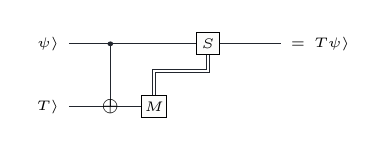
\begin{tikzpicture}[xscale=0.62, yscale=0.5,
          g/.style={draw, fill=paper, inner sep=1pt, minimum size=8pt, font=\tiny}]
        \node[font=\tiny, anchor=east] at (0.25,1.6) {$\ket{\psi}$};
        \node[font=\tiny, anchor=east] at (0.25,0) {$\ket{T}$};
        \draw[ink] (0.25,1.6) -- (4.6,1.6);
        \draw[ink] (0.25,0) -- (2.1,0);
        \filldraw[ink] (1.1,1.6) circle (1.3pt);
        \draw[ink] (1.1,1.6) -- (1.1,0);
        \node[font=\scriptsize] at (1.1,0) {$\oplus$};
        \node[g] at (2.0,0) {$M$};
        \draw[double, double distance=0.7pt, ink] (2.0,0.3) -- (2.0,0.9) -- (3.1,0.9) -- (3.1,1.35);
        \node[g] at (3.1,1.6) {$S$};
        \node[font=\tiny, anchor=west] at (4.6,1.6) {$=\,T\ket{\psi}$};
      \end{tikzpicture}\\[1pt]
      {\scriptsize\punch{$T$-gadget} --- the generality trick}\\
      {\tiny\color{mutedink} in-line $T$ $\to$ ancilla $+$ measurement $+$ conditional $S$ (hidden shift, 96 qubits)}\\[0.9em]
      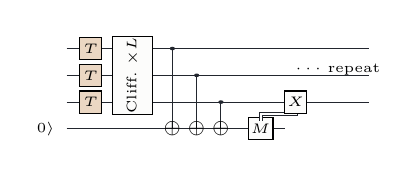
\begin{tikzpicture}[xscale=0.56, yscale=0.34,
          g/.style={draw, fill=paper, inner sep=1pt, minimum size=8pt, font=\tiny},
          t/.style={g, fill=copper!28}]
        \foreach \y in {1,2,3} \draw[ink] (0.55,\y) -- (7.4,\y);
        \draw[ink] (0.55,0) -- (5.5,0);
        \node[font=\tiny, anchor=east] at (0.5,0) {$\ket{0}$};
        \foreach \y in {1,2,3} \node[t] at (1.1,\y) {$T$};
        \draw[fill=paper] (1.6,0.55) rectangle (2.5,3.45);
        \node[rotate=90, font=\tiny] at (2.05,2) {Cliff.\ $\times L$};
        \foreach \x/\y in {2.95/3, 3.5/2, 4.05/1}{
          \filldraw[ink] (\x,\y) circle (1.3pt);
          \draw[ink] (\x,\y) -- (\x,0);
          \node[font=\scriptsize] at (\x,0) {$\oplus$};}
        \node[g] at (4.95,0) {$M$};
        \draw[double, double distance=0.7pt, ink] (4.95,0.3) -- (4.95,0.55) -- (5.75,0.55) -- (5.75,0.78);
        \node[g] at (5.75,1) {$X$};
        \node[font=\tiny] at (6.7,2.2) {$\cdots$ repeat};
      \end{tikzpicture}\\[1pt]
      {\scriptsize\punch{Cultivation patch} --- adaptive}\\
      {\tiny\color{mutedink} syndrome rounds $+$ logical Clifford traffic while magic accumulates (the frame's home turf)}
    \end{column}
  \end{columns}
  \takeaway{A stress test, a trick, a rhythm, a protocol --- each drives one benchmark.}
\end{frame}

% ================================================================ A: evidence
\begin{frame}{A \,\textperiodcentered\, Evidence (measured, against clifft's real fast path)}
  \begin{columns}[T]
    \begin{column}{0.55\textwidth}
      \begin{itemize}
        \item Everything validated to \punch{machine precision}; benchmarked against clifft's \emph{real} fast path.
        \item Crossover at \punch{$n\!\approx\!34$--$48$} (coarse--8\% error); past $n\!\approx\!62$ the \punch{only method that runs at all}.
        \item External tools: QuiZX $25\times$ slower by $n{=}56$; Quokka\# \punch{times out beyond $n{=}24$}.
      \end{itemize}
    \end{column}
    \begin{column}{0.42\textwidth}
      \small
      \begin{tabular}{@{}lrr@{}}
        \toprule
        $n=72$ & memory & time \\
        \midrule
        any exact method & $\sim$1 TB & --- \\
        \textcolor{copper}{\textbf{rank backend}} & \textcolor{copper}{\textbf{1.9 GB}} & \textcolor{copper}{\textbf{267 s}} \\
        \bottomrule
      \end{tabular}\\[1.0em]
      {\scriptsize\color{mutedink} Accuracy dial, measured:\\ error $=0.50\,\delta$ across the whole sweep\\ (halve the error $\Rightarrow$ $4\times$ the work).}
    \end{column}
  \end{columns}
  \takeaway{The niche is real --- and honestly bounded: below the crossover, exact clifft stays the right tool.}
\end{frame}

% ================================================================ A: runtimes
\begin{frame}{A \,\textperiodcentered\, Run times at a glance}
  \centering
  \small
  \begin{tabular}{@{}p{0.24\textwidth}p{0.44\textwidth}p{0.24\textwidth}@{}}
    \toprule
    \textbf{circuit family} & \textbf{measured head-to-head} & \textbf{cannot enter} \\
    \midrule
    dense IQP, $n{=}56$\newline\scriptsize(96 probabilities) &
    \textcolor{copper}{\textbf{rank backend 86\,s}} (8\% err) vs clifft exact 398\,s\newline
    {\scriptsize both exact: meet-in-the-middle 85\,s, QuiZX 2188\,s} &
    Quokka\# (timeout),\newline aer ($0/96$ in 455\,s) \\[2pt]
    dense IQP, $n{=}72$ &
    \textcolor{copper}{\textbf{rank backend 267\,s, 1.9\,GB}} &
    every exact method\newline($\sim$1\,TB) \\[2pt]
    hidden shift, 96 qubits &
    \textcolor{violet}{\textbf{clifft $\mu$s}} vs rank backend 8\,s --- dispatch picks clifft &
    --- \\[2pt]
    magic conveyor, 72 qubits &
    \textcolor{violet}{\textbf{clifft 1\,ms}} (block $=$ $2^{12}$) vs episodic 66\,s;\newline
    at width 128 (block $=$ $2^{49}$) \textcolor{copper}{\textbf{only episodic runs}} &
    whole-circuit rank backend\newline($2^{72}$ recipes) \\[2pt]
    cultivation patch (adaptive) &
    \textcolor{copper}{\textbf{frame $4$--$16\times$}} vs per-term engine &
    aer (rejects dynamic circuits) \\
    \bottomrule
  \end{tabular}
  \takeaway{No single winner --- that is the point: the dispatcher picks per program, before running.}
\end{frame}

% ================================================================ A: map
\begin{frame}{A \,\textperiodcentered\, Where it wins, where it doesn't}
  \centering
  \small
  \begin{tabular}{@{}p{0.30\textwidth}p{0.30\textwidth}p{0.30\textwidth}@{}}
    \toprule
    \textbf{Small peak rank} & \textbf{Large peak rank, sparse magic} & \textbf{Adaptive, Clifford-heavy} \\
    \midrule
    clifft is faster \emph{and} exact --- keep it. (Most circuits, however wide, compile here.) &
    \textcolor{copper}{\textbf{The niche}}: the only feasible method, accuracy dial-controlled. &
    \textcolor{copper}{\textbf{Real protocols win $2$--$16\times$}} --- and the standard open-source tool cannot run them at all. \\
    \bottomrule
  \end{tabular}
  \vspace{0.8em}
  \begin{itemize}
    \item Also measured where it \emph{loses} (up to $\sim\!2\times$ overhead) --- the advantage is a measured boundary, not a slogan.
  \end{itemize}
  \takeaway{Status: prototype validated; honest benchmarks, natural workloads, external baselines done.}
\end{frame}

% ================================================================ B: idea
\accentB
\begin{frame}{B \,\textperiodcentered\, The idea: don't run one shot faster --- run 4{,}096 abreast}
  \begin{columns}[T]
    \begin{column}{0.52\textwidth}
      \begin{itemize}
        \item One shot's small array \punch{cannot keep a GPU busy}: a stadium choir asked to sing one sentence.
        \item But workloads are \punch{thousands of shots} of the same program --- today run one after another.
        \item Put $B{=}4{,}096$ shots side by side; every gate hits \emph{all of them} in one launch.
      \end{itemize}
    \end{column}
    \begin{column}{0.44\textwidth}
      \centering
      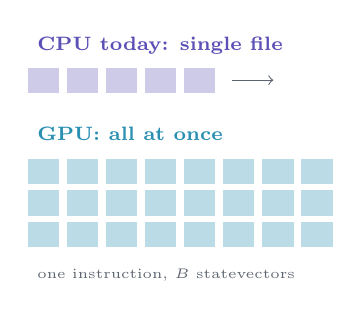
\begin{tikzpicture}[scale=0.8]
        % sequential CPU
        \node[font=\scriptsize\bfseries,color=violet,anchor=west] at (0,3.3) {CPU today: single file};
        \foreach \i in {0,1,2,3,4}{\fill[violet!30] (\i*0.62,2.55) rectangle (\i*0.62+0.5,2.95);}
        \draw[->,mutedink] (3.25,2.75) -- (3.9,2.75);
        % batched GPU
        \node[font=\scriptsize\bfseries,color=teal,anchor=west] at (0,1.9) {GPU: all at once};
        \foreach \i in {0,...,7}{\foreach \j in {0,1,2}{
          \fill[teal!32] (\i*0.62,1.5-\j*0.5) rectangle (\i*0.62+0.5,1.5-\j*0.5-0.4);}}
        \node[font=\tiny,color=mutedink,anchor=west] at (0,-0.35) {one instruction, $B$ statevectors};
      \end{tikzpicture}
    \end{column}
  \end{columns}
  \takeaway{Batching doesn't make the GPU faster --- it makes the problem big enough for the GPU to be fast.}
\end{frame}

% ================================================================ B: why 1
\begin{frame}{B \,\textperiodcentered\, Why it should work (1): shots march in lockstep}
  \begin{itemize}
    \item A shot's shape --- what runs when, how big the array is --- is \punch{identical for every shot}, fixed at compile time by clifft's compiler.
    \item Per-shot randomness is just a few numbers: \punch{SIMD lanes, one per shot}. The classic ``shots diverge'' objection \emph{does not apply here}.
    \item And nobody serves this niche: existing batched simulators \punch{fall back to one-at-a-time} on mid-circuit measurement --- clifft's home turf.
  \end{itemize}
  \takeaway{The hardest architectural question resolves in the design's favor before any GPU code is written.}
\end{frame}

% ================================================================ B: why 2
\begin{frame}{B \,\textperiodcentered\, Why it should work (2): the speed limit is bandwidth --- and GPUs have $7\times$ more}
  \begin{columns}[T]
    \begin{column}{0.52\textwidth}
      \begin{itemize}
        \item These kernels do almost no math per byte: \punch{memory speed is the speed limit}, on any machine.
        \item Measured: 11 CPU cores $=$ only $2.6\times$ one core --- the bus, not the cores.
        \item A GH200 has $\sim\!7\times$ the bandwidth $\Rightarrow$ \punch{5--10$\times$ more shots/s}, honestly bounded.
      \end{itemize}
    \end{column}
    \begin{column}{0.44\textwidth}
      \centering
      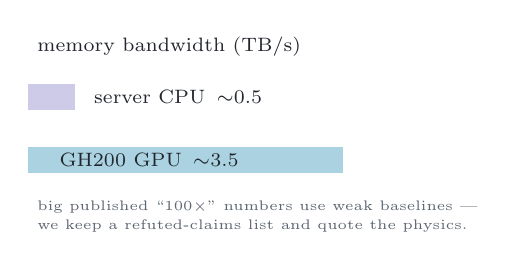
\begin{tikzpicture}[scale=0.8]
        \node[font=\scriptsize,color=ink,anchor=west] at (0,2.9) {memory bandwidth (TB/s)};
        \fill[violet!30] (0,1.9) rectangle (0.75,2.3);
        \node[font=\scriptsize,color=ink,anchor=west] at (0.9,2.1) {server CPU \,$\sim$0.5};
        \fill[teal!40] (0,0.9) rectangle (5.0,1.3);
        \node[font=\scriptsize,color=ink,anchor=west] at (0.35,1.1) {GH200 GPU \,$\sim$3.5};
        \node[font=\tiny,color=mutedink,anchor=west] at (0,0.35) {big published ``100$\times$'' numbers use weak baselines ---};
        \node[font=\tiny,color=mutedink,anchor=west] at (0,0.05) {we keep a refuted-claims list and quote the physics.};
      \end{tikzpicture}
    \end{column}
  \end{columns}
  \takeaway{The claim is deliberately modest --- which is why we can trust it.}
\end{frame}

% ================================================================ B: risk + test
\begin{frame}{B \,\textperiodcentered\, The one risk, and the \$20 experiment that settles it}
  \begin{itemize}
    \item Mid-circuit measurement needs the CPU: each crossing costs microseconds --- \punch{the same scale as the kernels themselves}.
    \item But it is paid \punch{once per batch} (nanoseconds per shot), on a link built to make it cheap.
    \item A faithful microbenchmark --- \emph{measurements and round-trips included} --- is built, validated, and waiting. \punch{GH200 time: \$2/hour.}
  \end{itemize}
  \centering
  {\small
  \begin{tabular}{@{}p{0.28\textwidth}p{0.64\textwidth}@{}}
    \toprule
    round-trip measured cheap & \textcolor{teal}{\textbf{go}}: batched backend; first target = replay-style queries (no round-trips at all) \\
    round-trip eats the win & \textbf{no-go}, cleanly --- or on-device sampling is the follow-up \\
    \bottomrule
  \end{tabular}}
  \takeaway{Either answer is cheap, quantitative, and final --- that is what the microbenchmark is for.}
\end{frame}

% ================================================================ closing
\accentO
\begin{frame}{How the two bets fit together}
  \begin{columns}[T]
    \begin{column}{0.46\textwidth}
      {\color{copper}\rule{0.5\textwidth}{2.2pt}}\\[0.3em]
      {\bfseries A \,\textperiodcentered\, Stabilizer rank extends \emph{reach}}\\[0.3em]
      {\small circuits clifft cannot hold at all today ---\\ approximate, with a measured accuracy dial}
    \end{column}
    \begin{column}{0.46\textwidth}
      {\color{teal}\rule{0.5\textwidth}{2.2pt}}\\[0.3em]
      {\bfseries B \,\textperiodcentered\, GPU batching extends \emph{throughput}}\\[0.3em]
      {\small the circuits clifft already runs ---\\ many more shots per second, exact as ever}
    \end{column}
  \end{columns}
  \vspace{1.2em}
  \begin{itemize}
    \item Both work \emph{because of} clifft's structure: the frame, the small block, the compile-time schedule.
    \item Both were reviewed adversarially; every headline number survived a fair baseline.
  \end{itemize}
  \vspace{0.4em}
  {\small\color{mutedink}\textbf{Next:} A --- benchmarks complete; write it up. \quad B --- the GH200 run, then batched replay queries.}
\end{frame}

\end{document}
